% Provenance (never printed): old seconde/premiere S material on the ocean
% (the ocean as a layered fluid, its heat, upwelling and productive waters);
% see sources/book2/PROVENANCE.md. All profiles are WOA23 columns, all
% densities the EOS-80 one-atmosphere equation, computed in
% figdata/grade-10/ocean_profiles.py.
\chapter{O oceano em camadas}\label{ch:g10:layered-ocean}

Num dia de verão, você nada a partir de uma praia numa água agradavelmente
morna. Depois deixa as pernas penderem --- e os seus pés encontram uma água
de repente fria, a um ou dois metros abaixo da superfície. O mar não é
misturado de cima a baixo: ele é feito de camadas, quentes e leves em cima,
frias e densas embaixo. No oceano aberto, essa mesma estrutura em camadas
desce por quilômetros, e é ela que decide onde o mar é um deserto e onde ele
fervilha de vida. Este capítulo olha o oceano em profundidade: como ele é
medido, como a sua temperatura e a sua salinidade mudam para baixo, por que
as camadas são estáveis, e onde a água fria profunda volta à superfície.

\begin{recall}
A água do mar contém sais dissolvidos: a sua salinidade, cerca de 35 gramas
de sal por quilograma de água do mar em média, varia de um mar para outro.
Os ventos movem as correntes de superfície e os grandes giros circulares;
correntes profundas de água fria e salgada se deslocam lentamente ao longo
do fundo do oceano (Livro 1, 8º ano). A densidade é a massa dividida pelo
volume (os livros de física). O fitoplâncton, algas microscópicas, precisa
de luz e de nutrientes minerais para crescer pela fotossíntese, e alimenta
o restante das cadeias alimentares do oceano (os livros de biologia).
\end{recall}

\section{Medir o oceano}

O oceano cobre cerca de \num{362}~milhões de~\unit{km^2} e tem em média
\qty{3682}{m} de profundidade: uns \num{1.33}~bilhão de~\unit{km^3} de água.
A maior parte dele fica muito abaixo do alcance da luz, e só pode ser medida
enviando instrumentos para baixo.
% ledger: charette:ocean-volume

De um navio, os oceanógrafos descem num cabo uma armação que leva sensores
que medem a condutividade da água (a partir da qual se calcula a sua
salinidade), a sua temperatura e a pressão (logo a profundidade), rodeados
por um anel de garrafas que são fechadas em profundidades escolhidas para
trazer amostras de água a bordo. Desde o ano 2000, uma frota de flutuadores
robóticos acrescentou milhões de perfis: cada flutuador deriva com as
correntes a uma profundidade de \qty{1000}{m}, afunda a cada dez dias, mais
ou menos, até \qty{2000}{m}, depois sobe até a superfície medindo a
temperatura e a salinidade no caminho, e envia o seu perfil por satélite.
% ledger: argo:fleet

\begin{dated}{2026}
A rede internacional Argo conta perto de 4000 flutuadores ativos; o seu
três milionésimo perfil foi coletado em julho de 2024.
% ledger: argo:fleet
\end{dated}

\begin{omfigure}
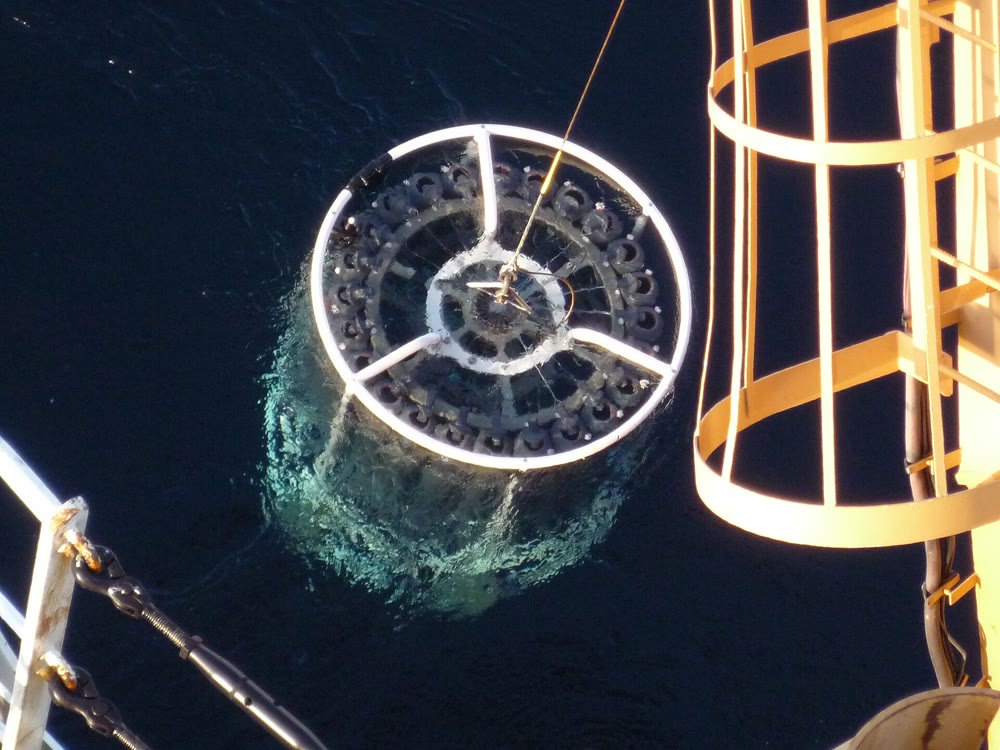
\includegraphics[height=4.4cm]{images/book2/g10-noaa-ctd-rosette.jpg}\hspace{0.4cm}%
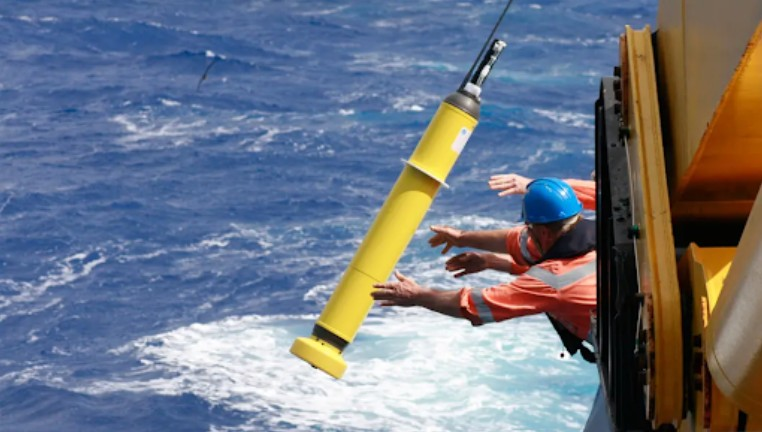
\includegraphics[height=4.4cm]{images/book2/g10-noaa-argo-float.jpg}

{\small À esquerda: uma roseta de garrafas de amostragem em torno dos seus
sensores, içada ao lado de um navio de pesquisa no Ártico, 2008 (fotografia:
Pablo Clemente-Colon, NOAA Photo Library). À direita: um flutuador
perfilador é lançado de um navio de pesquisa (fotografia: NOAA Global Ocean
Monitoring and Observing Program). Ambas em domínio público.}
\end{omfigure}

Em média sobre décadas de medições, esses perfis dão uma imagem do oceano em
profundidade. Os perfis deste capítulo são médias desse tipo, tiradas do
\emph{World Ocean Atlas 2023} dos NOAA National Centers for Environmental
Information.

\section{A temperatura com a profundidade}

\begin{omfigure}
\begin{tikzpicture}
\begin{axis}[omrecord, omdepth, width=0.62\linewidth, height=8.2cm,
  axis x line=top, xmin=-3, xmax=31, ymin=0, ymax=2000,
  xlabel={temperatura (\unit{\degreeCelsius})}, ylabel={profundidade (\unit{m})},
  tick label style={font=\small}, label style={font=\small},
  legend style={font=\scriptsize, at={(0.98,0.03)}, anchor=south east}]
\addplot[omThm!85!black, thick] table[x=t, y=depth] {figdata/out/grade-10-ocean_profiles-site-warmpool.dat};
\addplot[omDef!85!black, thick] table[x=t, y=depth] {figdata/out/grade-10-ocean_profiles-site-atlantic.dat};
\addplot[black!70, thick, dashed] table[x=t, y=depth] {figdata/out/grade-10-ocean_profiles-site-arctic.dat};
\legend{{Pacífico tropical, 5.5\textdegree N}, {Atlântico Norte, 40.5\textdegree N}, {Oceano Ártico, 75.5\textdegree N}}
\node[font=\scriptsize, anchor=west] (ml) at (axis cs:21,430) {\shortstack[l]{camada de\\mistura}};
\draw[black!50] (ml.north east) -- (axis cs:28.9,35);
\node[font=\scriptsize, anchor=west] (tc) at (axis cs:15.5,600) {termoclina};
\draw[black!50] (tc.north) -- (axis cs:19.9,150);
\node[font=\scriptsize, anchor=west] at (axis cs:7,1500) {oceano profundo};
\end{axis}
\end{tikzpicture}

{\small Temperatura média em função da profundidade em três locais (a
profundidade aumenta para baixo). Dados: World Ocean Atlas 2023, médias
anuais, NOAA NCEI.}
\end{omfigure}
% ledger: data:b2-woa23 (profiles in figdata/grade-10/ocean_profiles.py)

A luz do Sol aquece o oceano por cima, na sua camada de superfície. O vento
e as ondas misturam essa água quente numa camada de temperatura quase
uniforme. Abaixo dela, a temperatura cai depressa ao longo de algumas
centenas de metros; mais fundo ainda, ela cai devagar até a água fria que
enche as bacias oceânicas.

\begin{definition}[Camada de mistura]\label{def:g10:layered-ocean:mixed-layer}
A \emph{camada de mistura}\index{camada de mistura} é a camada de superfície
do oceano, misturada pelo vento e pelas ondas, na qual a temperatura e a
salinidade quase não mudam com a profundidade.
\end{definition}

\begin{definition}[Termoclina; haloclina; picnoclina; oceano profundo]\label{def:g10:layered-ocean:thermocline}
A \emph{termoclina}\index{termoclina} é a camada abaixo da \omterm{def:g10:layered-ocean:mixed-layer}{camada de mistura}
na qual a temperatura cai depressa com a profundidade. A camada na qual a
salinidade muda depressa com a profundidade é uma
\emph{haloclina}\index{haloclina}; a camada na qual a densidade aumenta
depressa com a profundidade é a \emph{picnoclina}\index{picnoclina}. Abaixo
delas fica o \emph{oceano profundo}\index{oceano profundo}, frio e de
mudança lenta.
\end{definition}

No Pacífico tropical, a \omterm{def:g10:layered-ocean:mixed-layer}{camada de mistura} está a \qty{29.2}{\degreeCelsius}
e tem uns \qty{60}{m} de espessura; entre \qty{70}{m} e \qty{300}{m}, a
temperatura cai quase dezenove graus, e a \qty{1000}{m} ela já desceu a
\qty{4.5}{\degreeCelsius}. No Atlântico Norte, a superfície é mais fresca e
a queda mais gradual. No Oceano Ártico, a coluna inteira fica a menos de
dois graus de \qty{0}{\degreeCelsius}: não há, por assim dizer, camada
quente de superfície.
% ledger: data:b2-woa23

\begin{method}[Ler um perfil oceânico]\label{met:g10:layered-ocean:profile}
\begin{enumerate}
  \item Encontre os eixos: a profundidade aumenta para baixo, a grandeza
        medida é lida ao longo do topo.
  \item A \omterm{def:g10:layered-ocean:mixed-layer}{camada de mistura} é a parte de cima, onde a curva é quase
        vertical; a sua profundidade é onde a curva começa a se afastar da
        vertical (uma regra comum: onde a temperatura caiu
        \qty{0.5}{\degreeCelsius} abaixo do seu valor na superfície).
  \item A \omterm{def:g10:layered-ocean:thermocline}{termoclina} é onde a curva está mais perto da horizontal: a maior
        mudança para a menor profundidade.
  \item Mais abaixo, leia os valores profundos e compare os locais na mesma
        profundidade.
\end{enumerate}
\end{method}

A \omterm{def:g10:layered-ocean:mixed-layer}{camada de mistura} muda com as estações. No inverno, a superfície perde
calor, as tempestades agitam o mar e a \omterm{def:g10:layered-ocean:mixed-layer}{camada de mistura} se aprofunda; no
verão, o sol aquece uma fina camada de superfície que os ventos mais suaves
não conseguem misturar para baixo, e uma \emph{\omterm{def:g10:layered-ocean:thermocline}{termoclina} sazonal} se forma
perto da superfície --- a água fria que os pés do nadador encontram.

\begin{omfigure}
\begin{tikzpicture}
\begin{axis}[omrecord, omdepth, width=0.6\linewidth, height=6.6cm,
  axis x line=top, xmin=12, xmax=24, ymin=0, ymax=300,
  xlabel={temperatura (\unit{\degreeCelsius})}, ylabel={profundidade (\unit{m})},
  tick label style={font=\small}, label style={font=\small},
  legend style={font=\scriptsize, at={(0.98,0.03)}, anchor=south east}]
\addplot[omDef!85!black, thick] table[x=t_feb, y=depth] {figdata/out/grade-10-ocean_profiles-season.dat};
\addplot[omThm!85!black, thick] table[x=t_aug, y=depth] {figdata/out/grade-10-ocean_profiles-season.dat};
\legend{fevereiro, agosto}
\end{axis}
\end{tikzpicture}

{\small Inverno e verão no Atlântico Norte (40.5\textdegree N,
30.5\textdegree O): temperaturas médias mensais de fevereiro e de agosto.
Em fevereiro, a \omterm{def:g10:layered-ocean:mixed-layer}{camada de mistura} chega a cerca de \qty{170}{m}; em agosto,
uma camada quente de cerca de \qty{15}{m} de espessura repousa sobre uma
\omterm{def:g10:layered-ocean:thermocline}{termoclina} sazonal. Dados: World Ocean Atlas 2023, NOAA NCEI.}
\end{omfigure}
% ledger: data:b2-woa23 (mixed-layer depths by the 0.5 degC rule, computed in figdata/grade-10/ocean_profiles.py)

\section{Salinidade e densidade}

A densidade da água do mar depende da sua temperatura e da sua salinidade.
Ela é calculada por uma fórmula acordada internacionalmente, a equação de
estado da água do mar, ajustada a medições de laboratório.

\begin{proposition}[Densidade da água do mar]\label{prop:g10:layered-ocean:density}
A densidade da água do mar aumenta com a sua salinidade e diminui quando a
sua temperatura sobe. À pressão da superfície, a água do mar de salinidade
35 tem uma densidade de \qty{1028.1}{kg/m^3} a \qty{0}{\degreeCelsius} e de
\qty{1023.3}{kg/m^3} a \qty{25}{\degreeCelsius}; a água pura a
\qty{4}{\degreeCelsius} tem uma densidade de \qty{1000.0}{kg/m^3}.
\end{proposition}
% ledger: unesco:eos80 (values computed in figdata/grade-10/ocean_profiles.py)

\begin{omfigure}
\begin{tikzpicture}
\begin{axis}[omrecord, width=0.7\linewidth, height=6.2cm, xmin=-2, xmax=30,
  ymin=1016, ymax=1033, xlabel={temperatura (\unit{\degreeCelsius})},
  ylabel={densidade (\unit{kg/m^3})}, tick label style={font=\small},
  label style={font=\small}, yticklabel style={/pgf/number format/1000 sep={}}]
\addplot[omThm!85!black, thick] table[x=t, y=rho_s38] {figdata/out/grade-10-ocean_profiles-eos.dat};
\addplot[black!80, thick] table[x=t, y=rho_s35] {figdata/out/grade-10-ocean_profiles-eos.dat};
\addplot[omDef!85!black, thick] table[x=t, y=rho_s30] {figdata/out/grade-10-ocean_profiles-eos.dat};
\node[font=\scriptsize, anchor=south west, omThm!85!black] at (axis cs:1,1030.75) {salinidade 38};
\node[font=\scriptsize, anchor=south west] at (axis cs:1,1028.35) {salinidade 35};
\node[font=\scriptsize, anchor=south west, omDef!85!black] at (axis cs:1,1024.35) {salinidade 30};
\end{axis}
\end{tikzpicture}

{\small A densidade da água do mar à pressão da superfície, em função da sua
temperatura, para três salinidades (calculada pela equação de estado
internacional da água do mar).}
\end{omfigure}
% ledger: unesco:eos80

Duas coisas aparecem no gráfico. Uma unidade de salinidade acrescenta cerca
de \qty{0.8}{kg/m^3}. Um grau de aquecimento retira cerca de
\qty{0.31}{kg/m^3} a \qty{25}{\degreeCelsius}, \qty{0.18}{kg/m^3} a
\qty{10}{\degreeCelsius}, mas apenas \qty{0.06}{kg/m^3} perto de
\qty{0}{\degreeCelsius}: nos mares quentes, é a temperatura que controla a
densidade; nos mares frios, é a salinidade.
% ledger: unesco:eos80 (slopes computed in figdata/grade-10/ocean_profiles.py)

\begin{remark}
As densidades deste capítulo são calculadas à pressão da superfície. A
pressão da água de cima comprime um pouco a água do mar, cerca de
\qty{4}{kg/m^3} por quilômetro de profundidade; os oceanógrafos comparam as
massas de água à mesma pressão, para que só a temperatura e a salinidade
contem.
\end{remark}
% ledger: unesco:eos80-checks (computed in figdata/grade-10/ocean_profiles.py: 3.9 kg/m3 per km from the 10000-dbar check values)

\begin{omfigure}
\begin{tikzpicture}
\begin{axis}[name=sal, omrecord, omdepth, width=0.5\linewidth, height=7.2cm,
  axis x line=top, xmin=27.5, xmax=37, ymin=0, ymax=1000,
  xlabel={salinidade}, ylabel={profundidade (\unit{m})},
  tick label style={font=\small}, label style={font=\small}]
\addplot[omThm!85!black, thick] table[x=s, y=depth] {figdata/out/grade-10-ocean_profiles-site-warmpool.dat};
\addplot[omDef!85!black, thick] table[x=s, y=depth] {figdata/out/grade-10-ocean_profiles-site-atlantic.dat};
\addplot[black!70, thick, dashed] table[x=s, y=depth] {figdata/out/grade-10-ocean_profiles-site-arctic.dat};
\node[font=\scriptsize, anchor=west, align=left] at (axis cs:28.2,120) {haloclina\\do Ártico};
\end{axis}
\begin{axis}[at={(sal.east)}, anchor=west, xshift=0.9cm, omrecord, omdepth,
  width=0.5\linewidth, height=7.2cm, axis x line=top, xmin=1021, xmax=1028.5, yticklabels={},
  ymin=0, ymax=1000, xlabel={densidade (\unit{kg/m^3})},
  tick label style={font=\small}, label style={font=\small},
  xticklabel style={/pgf/number format/1000 sep={}},
  legend style={font=\scriptsize, at={(0.03,0.03)}, anchor=south west}]
\addplot[omThm!85!black, thick] table[x=rho, y=depth] {figdata/out/grade-10-ocean_profiles-site-warmpool.dat};
\addplot[omDef!85!black, thick] table[x=rho, y=depth] {figdata/out/grade-10-ocean_profiles-site-atlantic.dat};
\addplot[black!70, thick, dashed] table[x=rho, y=depth] {figdata/out/grade-10-ocean_profiles-site-arctic.dat};
\legend{Pacífico tropical, Atlântico Norte, Oceano Ártico}
\end{axis}
\end{tikzpicture}

{\small Salinidade (à esquerda) e densidade à pressão da superfície (à
direita) em função da profundidade, nos três locais dos perfis de
temperatura. Em todos os locais, a densidade aumenta para baixo. Dados:
World Ocean Atlas 2023, NOAA NCEI; densidades pela equação de estado
internacional da água do mar.}
\end{omfigure}
% ledger: data:b2-woa23, unesco:eos80

No Pacífico tropical, a \omterm{def:g10:layered-ocean:thermocline}{picnoclina} coincide com a \omterm{def:g10:layered-ocean:thermocline}{termoclina}. No Oceano
Ártico, a temperatura quase não muda, mas a salinidade sobe de 28 na
superfície, adoçada pelos rios e pelo gelo que derrete, a 34.8 a
\qty{500}{m}: a \omterm{def:g10:layered-ocean:thermocline}{haloclina} é a \omterm{def:g10:layered-ocean:thermocline}{picnoclina}. Em cada caso, a densidade aumenta
para baixo.
% ledger: data:b2-woa23

\begin{definition}[Estratificação]\label{def:g10:layered-ocean:stratification}
O oceano está \emph{estratificado}\index{estratificacao@estratificação}
quando a sua densidade aumenta com a profundidade: água mais leve repousa
sobre água mais densa, em camadas.
\end{definition}

Um oceano \omterm{def:g10:layered-ocean:stratification}{estratificado} é estável. Uma parcela de água empurrada para baixo,
para dentro de uma água mais densa, é mais leve que o seu entorno e volta a
flutuar para cima; uma parcela empurrada para cima volta a afundar. Para
misturar as camadas, o vento precisa trabalhar contra isso, e quanto mais
forte a \omterm{def:g10:layered-ocean:thermocline}{picnoclina}, mais difícil é: a \omterm{def:g10:layered-ocean:thermocline}{termoclina} é uma tampa que separa a
superfície do \omterm{def:g10:layered-ocean:thermocline}{oceano profundo}. O \omterm{def:g10:layered-ocean:thermocline}{oceano profundo} é preenchido por água que
afundou há muito tempo nos mares polares frios, onde a água de superfície
fica densa o bastante para afundar (Livro 1, 8º ano).

\section{A ressurgência}

\begin{definition}[Ressurgência]\label{def:g10:layered-ocean:upwelling}
A \emph{ressurgência}\index{ressurgencia@ressurgência} é a subida de água
fria de baixo da camada de superfície, para substituir a água de superfície
que o vento empurra para longe. Ela ocorre ao longo de algumas costas e em
oceano aberto.
\end{definition}
% ledger: noaa:upwelling

Ao longo de uma costa, o vento que sopra paralelo à orla arrasta a água de
superfície; por causa da rotação da Terra, a água não segue simplesmente o
vento, mas é desviada dele, para a direita no Hemisfério Norte e para a
esquerda no Hemisfério Sul (como isso funciona é o assunto dos volumes
universitários). Ao largo do Peru, o vento sopra ao longo da costa em
direção ao equador, e a água de superfície é empurrada para o mar aberto; a
água fria sobe perto da costa para tomar o seu lugar. A \omterm{def:g10:layered-ocean:upwelling}{ressurgência} também
ocorre ao longo do equador, onde os ventos alísios afastam dele a água de
superfície dos dois lados.
% ledger: noaa:upwelling, kessler:peru-upwelling

\begin{omfigure}
\begin{tikzpicture}[font=\footnotesize, >={Stealth[length=2mm]}]
  % ocean and thermocline
  \fill[omDef!12] (0,-3.2) rectangle (8.2,0);
  \fill[omDef!30] (0,-3.2) -- (0,-2.0) .. controls (3,-2.0) and (5.5,-1.6) .. (7.4,-0.35) -- (8.2,0) -- (8.2,-3.2) -- cycle;
  \draw[omDef!80!black, dashed] (0,-2.0) .. controls (3,-2.0) and (5.5,-1.6) .. (7.4,-0.35);
  \node[anchor=north west, omDef!80!black] at (0.1,-2.05) {termoclina};
  \node[anchor=west, black!70] at (0.15,-0.9) {água quente de superfície};
  \node[anchor=west, black!70] at (0.15,-2.75) {água fria, rica em nutrientes};
  % land
  \fill[omExo!30, draw=black!60] (7.0,-3.2) -- (8.2,-0.1) -- (8.6,0.0) -- (9.6,1.2) -- (10.6,2.2) -- (10.6,-3.2) -- cycle;
  \node[anchor=south, align=center] at (9.9,-1.6) {terra};
  % surface flow and rising water
  \draw[->, thick, omThm!80!black] (7.2,-0.3) -- (3.6,-0.3);
  \node[anchor=south, omThm!80!black] at (5.4,-0.25) {água de superfície levada ao largo};
  \foreach \x/\y in {6.1/-2.1, 6.8/-1.7} \draw[->, thick, omDef!80!black] (\x,\y) -- (\x+0.45,\y+1.15);
  \node[anchor=north, omDef!80!black, align=center] at (6.0,-2.25) {a água fria sobe};
  % wind along the shore, northward: with west on the left and east on the
  % right the reader looks north, so the wind goes into the page
  \draw[black!70, thick] (2.6,1.0) circle (0.22);
  \draw[black!70, thick] (2.6,1.0) ++(45:0.22) -- ++(225:0.44) (2.6,1.0) ++(135:0.22) -- ++(315:0.44);
  \node[anchor=west, align=left] at (2.9,1.0) {vento ao longo da costa, rumo ao equador\\(para o norte, para dentro da página)};
  \node[anchor=north west, black!60] at (0,-3.25) {$\leftarrow$ oeste};
  \node[anchor=north east, black!60] at (10.6,-3.25) {leste $\rightarrow$};
\end{tikzpicture}

{\small \omterm{def:g10:layered-ocean:upwelling}{Ressurgência} costeira ao largo do Peru (corte esquemático de oeste
para leste, fora de escala): o vento sopra ao longo da costa em direção ao
equador, para o norte, para dentro da página; a água de superfície é desviada
para a sua esquerda e empurrada para o mar aberto; a água fria de baixo da
\omterm{def:g10:layered-ocean:thermocline}{termoclina} sobe perto da costa para substituí-la.}
\end{omfigure}

A água que sobe não é apenas fria. Abaixo da camada de superfície
iluminada, os restos do plâncton morto que afundam e se decompõem liberam os
nutrientes minerais de que o fitoplâncton precisa. Trazidos de volta para a
luz, esses nutrientes fazem das regiões de \omterm{def:g10:layered-ocean:upwelling}{ressurgência} as águas mais
produtivas do oceano, com os pesqueiros mais ricos. Onde o oceano é
fortemente \omterm{def:g10:layered-ocean:stratification}{estratificado} e nada traz água profunda para cima, a camada
iluminada fica sem nutrientes: os centros dos giros subtropicais são os
desertos do oceano.
% ledger: noaa:upwelling

\begin{omfigure}
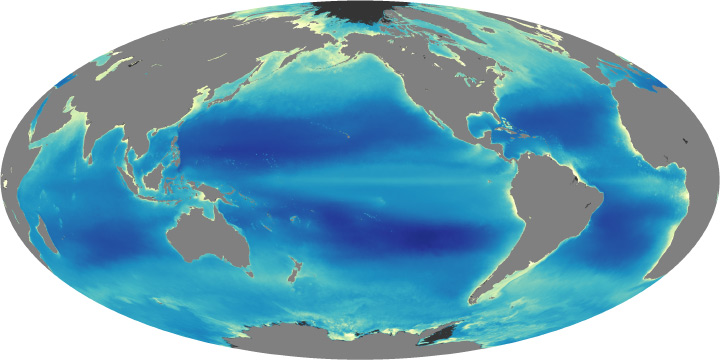
\includegraphics[width=0.8\linewidth]{images/book2/g10-nasa-ocean-chlorophyll.jpg}

{\small A clorofila do fitoplâncton vista do espaço, em média sobre
2002--2010: do azul-escuro (muito pouca), passando pelo azul-claro, até o
amarelo (muita); terra em cinza. A costa do Peru e a faixa ao longo do
equador no Pacífico se destacam; os giros são de um azul profundo. Imagem:
Jesse Allen e Robert Simmon, NASA Earth Observatory (domínio público).}
\end{omfigure}

\begin{omfigure}
\begin{tikzpicture}
\begin{axis}[omrecord, omdepth, width=0.6\linewidth, height=7.2cm,
  axis x line=top, xmin=4, xmax=26, ymin=0, ymax=600,
  xlabel={temperatura (\unit{\degreeCelsius})}, ylabel={profundidade (\unit{m})},
  tick label style={font=\small}, label style={font=\small},
  legend style={font=\scriptsize, at={(0.98,0.03)}, anchor=south east}]
\addplot[omExo!85!black, thick] table[x=t, y=depth] {figdata/out/grade-10-ocean_profiles-site-peru.dat};
\addplot[omThm!85!black, thick] table[x=t, y=depth] {figdata/out/grade-10-ocean_profiles-site-gyre.dat};
\addplot[black!40, dashed, domain=0:600, samples=2] ({15}, {x});
\legend{{ao largo do Peru, 13.5\textdegree S}, {giro do Pacífico Sul, 20.5\textdegree S}}
\end{axis}
\end{tikzpicture}

{\small Ao largo do Peru, a água fria chega perto da superfície: a água a
\qty{15}{\degreeCelsius} (linha tracejada) fica a cerca de \qty{65}{m},
contra quase \qty{300}{m} no meio do giro do Pacífico Sul, que fica mais
longe do equador. Dados: World Ocean Atlas 2023, médias anuais, NOAA NCEI.}
\end{omfigure}
% ledger: data:b2-woa23

\section{Exercícios}

\begin{exercise}[$\star$]\label{exo:g10:layered-ocean:1}
Defina a \omterm{def:g10:layered-ocean:mixed-layer}{camada de mistura} e a \omterm{def:g10:layered-ocean:thermocline}{termoclina}. O que agita a \omterm{def:g10:layered-ocean:mixed-layer}{camada de mistura}?
\end{exercise}

\begin{exercise}[$\star$]\label{exo:g10:layered-ocean:2}
Defina a \omterm{def:g10:layered-ocean:upwelling}{ressurgência}. Por que as águas das regiões de \omterm{def:g10:layered-ocean:upwelling}{ressurgência} são ricas
em vida?
\end{exercise}

\begin{exercise}[$\star$]\label{exo:g10:layered-ocean:3}
Usando os perfis de temperatura dos três locais, dê a temperatura na
superfície e a \qty{1000}{m} no Pacífico tropical e no Oceano Ártico.
\end{exercise}

\begin{exercise}[$\star$]\label{exo:g10:layered-ocean:4}
O que é mais denso: a água do mar de salinidade 35 a \qty{25}{\degreeCelsius}
ou a \qty{0}{\degreeCelsius}? A água do mar de salinidade 35 ou a água pura,
à mesma temperatura? Use os valores do capítulo.
\end{exercise}

\begin{exercise}[$\star$]\label{exo:g10:layered-ocean:5}
Explique como um flutuador perfilador mede um perfil do oceano, e por que os
flutuadores são úteis onde os navios raramente vão.
\end{exercise}

\begin{exercise}[$\star\star$]\label{exo:g10:layered-ocean:6}
O oceano cobre \num{361.84}~milhões de~\unit{km^2}, com uma profundidade
média de \qty{3682}{m}. Calcule o seu volume em quilômetros cúbicos. Que
fração da sua profundidade representam os \qty{100}{m} de cima?
\end{exercise}

\begin{exercise}[$\star\star$]\label{exo:g10:layered-ocean:7}
No perfil de agosto do Atlântico Norte, a temperatura é de
\qty{22.7}{\degreeCelsius} na superfície, \qty{22.2}{\degreeCelsius} a
\qty{15}{m}, \qty{21.8}{\degreeCelsius} a \qty{20}{m} e
\qty{17.3}{\degreeCelsius} a \qty{50}{m}. Usando a regra do método, estime
a profundidade da \omterm{def:g10:layered-ocean:mixed-layer}{camada de mistura}. Qual é a taxa média de queda da
temperatura entre \qty{20}{m} e \qty{50}{m}, em graus por metro?
\end{exercise}

\begin{exercise}[$\star\star$]\label{exo:g10:layered-ocean:8}
No mesmo local do Atlântico Norte, a superfície está a
\qty{15.3}{\degreeCelsius} em fevereiro e a \qty{22.7}{\degreeCelsius} em
agosto, enquanto a \qty{300}{m} ela está a \qty{13.5}{\degreeCelsius} nos
dois meses. Explique por que a água profunda não acompanha as estações, e
por que a \omterm{def:g10:layered-ocean:mixed-layer}{camada de mistura} de inverno é muito mais profunda que a de verão.
\end{exercise}

\begin{exercise}[$\star\star$]\label{exo:g10:layered-ocean:9}
Perto de \qty{10}{\degreeCelsius}, uma unidade de salinidade acrescenta
\qty{0.78}{kg/m^3} à densidade e um grau de aquecimento retira
\qty{0.18}{kg/m^3}. Quantos graus de aquecimento anulam uma unidade de
salinidade? Responda à mesma pergunta perto de \qty{0}{\degreeCelsius}, onde
um grau retira apenas \qty{0.06}{kg/m^3}. O que você conclui para os mares
polares?
\end{exercise}

\begin{exercise}[$\star\star$]\label{exo:g10:layered-ocean:10}
No Oceano Ártico, a água da superfície está a \qty{-1.4}{\degreeCelsius}
com uma salinidade de 28.1, e a \qty{200}{m} ela está a
\qty{-1.4}{\degreeCelsius} com uma salinidade de 33.3. As suas densidades são
\qty{1022.6}{kg/m^3} e \qty{1026.8}{kg/m^3}. O que torna a água mais funda
mais densa? Dê o nome da camada entre elas.
\end{exercise}

\begin{exercise}[$\star\star$]\label{exo:g10:layered-ocean:11}
Explique por que um oceano \omterm{def:g10:layered-ocean:stratification}{estratificado} é estável, usando uma parcela de
água de superfície empurrada para baixo por uma onda.
\end{exercise}

\begin{exercise}[$\star\star\star$]\label{exo:g10:layered-ocean:12}
Um litro de água do mar de salinidade 35 a \qty{0}{\degreeCelsius} é
aquecido até \qty{25}{\degreeCelsius}. Usando as densidades do capítulo,
calcule a sua massa, depois o seu novo volume. Quanto ele se dilatou, em
mililitros? Uma camada de oceano de \qty{700}{m} de espessura se aquece na
mesma proporção: quanto cresce a sua espessura? (Isto é um grande exagero do
aquecimento real do oceano, usado aqui apenas para mostrar o efeito.)
\end{exercise}

\begin{exercise}[$\star\star\star$]\label{exo:g10:layered-ocean:13}
No Pacífico tropical, a densidade é de \qty{1021.6}{kg/m^3} a \qty{50}{m} e
de \qty{1026.0}{kg/m^3} a \qty{200}{m}; no Atlântico Norte, em fevereiro, a
temperatura quase não muda nos \qty{150}{m} de cima. Em qual dos dois uma
tempestade teria mais facilidade para misturar a água até \qty{150}{m}?
Explique.
\end{exercise}

\begin{exercise}[$\star\star\star$]\label{exo:g10:layered-ocean:14}
No mapa da clorofila, encontre duas regiões de clorofila alta em oceano
aberto, longe de qualquer costa, e uma grande região de clorofila muito
baixa. Usando o capítulo, explique cada uma.
\end{exercise}

\begin{exercise}[$\star\star\star$]\label{exo:g10:layered-ocean:15}
Suponha que um flutuador afunde de \qty{1000}{m} a \qty{2000}{m} em seis
horas, depois suba até a superfície em dez horas. Calcule a sua velocidade
vertical média em cada fase, em centímetros por segundo. Se ele medisse a
cada \qty{2}{s} durante a subida, quantas medições conteria um perfil, e que
profundidade separa duas delas em média?
\end{exercise}

\section{Problema: uma sondagem ao largo do Peru}

\begin{problem}[{Problema de fim de semana --- dois perfis do Pacífico Sul}]
\label{pb:g10:layered-ocean:1}
% ledger: data:b2-woa23, unesco:eos80 (values rounded from figdata/grade-10/ocean_profiles.py)
A tabela dá a temperatura e a salinidade médias, e a densidade calculada à
pressão da superfície, em dois lugares do Pacífico Sul: ao largo do Peru
(\qty{13.5}{\degree S}, \qty{77.5}{\degree O}) e no meio do giro
subtropical (\qty{20.5}{\degree S}, \qty{110.5}{\degree O}).

\begin{center}
\small
\begin{tabular}{c|ccc|ccc}
\hline
 & \multicolumn{3}{c|}{ao largo do Peru} & \multicolumn{3}{c}{giro} \\
profundidade (\unit{m}) & \unit{\degreeCelsius} & salinidade & \unit{kg/m^3} & \unit{\degreeCelsius} & salinidade & \unit{kg/m^3} \\
\hline
0 & 19.0 & 35.08 & 1025.08 & 24.0 & 36.41 & 1024.71 \\
25 & 17.4 & 35.06 & 1025.47 & 23.9 & 36.39 & 1024.73 \\
50 & 15.8 & 35.03 & 1025.83 & 23.6 & 36.38 & 1024.80 \\
100 & 13.7 & 34.93 & 1026.20 & 22.6 & 36.27 & 1025.02 \\
200 & 12.4 & 34.89 & 1026.44 & 20.3 & 35.80 & 1025.30 \\
300 & 11.1 & 34.80 & 1026.62 & 14.4 & 34.76 & 1025.92 \\
500 & 7.9 & 34.60 & 1026.97 & 7.1 & 34.39 & 1026.92 \\
\hline
\end{tabular}
\end{center}

\medskip
\noindent\textbf{Parte I --- Ler os perfis.}
\begin{enumerate}
  \item Qual local é mais quente na superfície, e por quanto?
  \item Qual local fica mais longe do equador? A diferença de temperatura de
        superfície é a que você esperaria só pelas latitudes?
  \item Usando a regra do método, estime a profundidade da \omterm{def:g10:layered-ocean:mixed-layer}{camada de mistura}
        no giro.
  \item Há uma \omterm{def:g10:layered-ocean:mixed-layer}{camada de mistura} ao largo do Peru? Descreva os \qty{100}{m}
        de cima.
  \item Entre quais profundidades a temperatura cai mais depressa no giro?
        Dê a taxa, em graus por cem metros.
  \item A que profundidade, aproximadamente, a água está a
        \qty{15}{\degreeCelsius} em cada local?
\end{enumerate}

\medskip
\noindent\textbf{Parte II --- As densidades.}
\begin{enumerate}[resume]
  \item Verifique que a densidade aumenta com a profundidade nos dois locais.
        O que isso diz sobre a sua estabilidade?
  \item No giro, a água de superfície é mais salgada que ao largo do Peru.
        Isso deveria torná-la mais densa ou mais leve? Ela é mais densa?
  \item Explique qual dos dois efeitos vence.
  \item Calcule o aumento de densidade da superfície até \qty{200}{m} ao
        largo do Peru.
  \item Calcule o mesmo aumento no giro.
\end{enumerate}

\medskip
\noindent\textbf{Parte III --- A estratificação comparada.}
\begin{enumerate}[resume]
  \item No giro, onde se encontra a maior parte do aumento de densidade dos
        \qty{500}{m} de cima: acima ou abaixo de \qty{200}{m}?
  \item E ao largo do Peru, onde ela se encontra?
  \item A \qty{500}{m}, compare os dois locais. O que isso sugere sobre a
        água profunda abaixo de ambos?
  \item Explique em algumas frases como a \omterm{def:g10:layered-ocean:thermocline}{termoclina} ao largo do Peru foi
        levantada em direção à superfície.
  \item O fitoplâncton vive nas primeiras dezenas de metros. Em qual local a
        água rica em nutrientes de baixo da \omterm{def:g10:layered-ocean:thermocline}{termoclina} está ao alcance da
        agitação pelo vento? Explique.
\end{enumerate}

\medskip
\noindent\textbf{Parte IV --- Por que as águas peruanas são produtivas.}
\begin{enumerate}[resume]
  \item Como seria a água de superfície ao largo do Peru se o vento ao longo
        da costa parasse de soprar durante meses?
  \item Usando o mapa da clorofila, compare os dois locais.
  \item Explique por que o giro é chamado de deserto do oceano, embora seja
        cheio de luz do Sol.
  \item Calcule a razão entre os aumentos de densidade da superfície até
        \qty{200}{m} ao largo do Peru e no giro, e diga o que ela mostra.
\end{enumerate}
\end{problem}
